\documentclass[12pt]{article}
\usepackage[utf8]{inputenc}
\usepackage[a4paper,margin=1in]{geometry}
\usepackage{amsmath,amssymb}
\usepackage{enumitem}
\usepackage{parskip}
\usepackage{hyperref}
\usepackage{xcolor}
\usepackage{fancyhdr}
\usepackage{tikz}
\usepackage{graphicx}
\usepackage{eso-pic}
\usepackage{titlesec}

\graphicspath{{../}}

\definecolor{kcpc-bg}{RGB}{250,250,250}
\definecolor{kcpc-text}{RGB}{20,20,20}
\definecolor{kcpc-muted}{RGB}{90,90,90}
\definecolor{kcpc-red}{RGB}{176,0,0}

\newcommand{\kcpcwordmark}{\raisebox{-0.15\height}{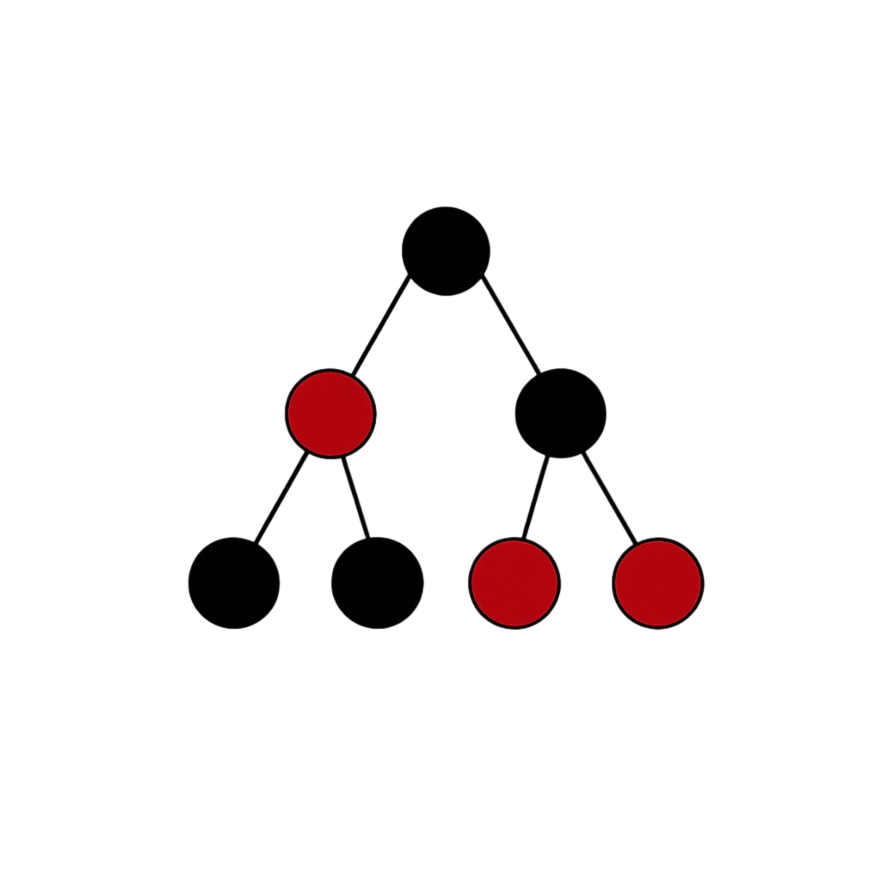
\includegraphics[height=0.55cm]{kcpc-logo.png}}}

\pagestyle{fancy}
\fancyhf{}
\lhead{\textcolor{kcpc-text}{\small\bfseries Problems}}
\rhead{\textcolor{kcpc-muted}{\small Week 1}}
\cfoot{\textcolor{kcpc-muted}{\small KCPC}}
\renewcommand{\headrulewidth}{0.4pt}
\renewcommand{\headrule}{\hbox
to\headwidth{\color{kcpc-red}\leaders\hrule height \headrulewidth\hfill}}
\renewcommand{\footrulewidth}{0pt}
\setlength{\headheight}{28pt}

\AddToShipoutPictureBG{%
    \begin{tikzpicture}[remember picture,overlay]
        \node[opacity=0.035, at=(current page.center)]
        {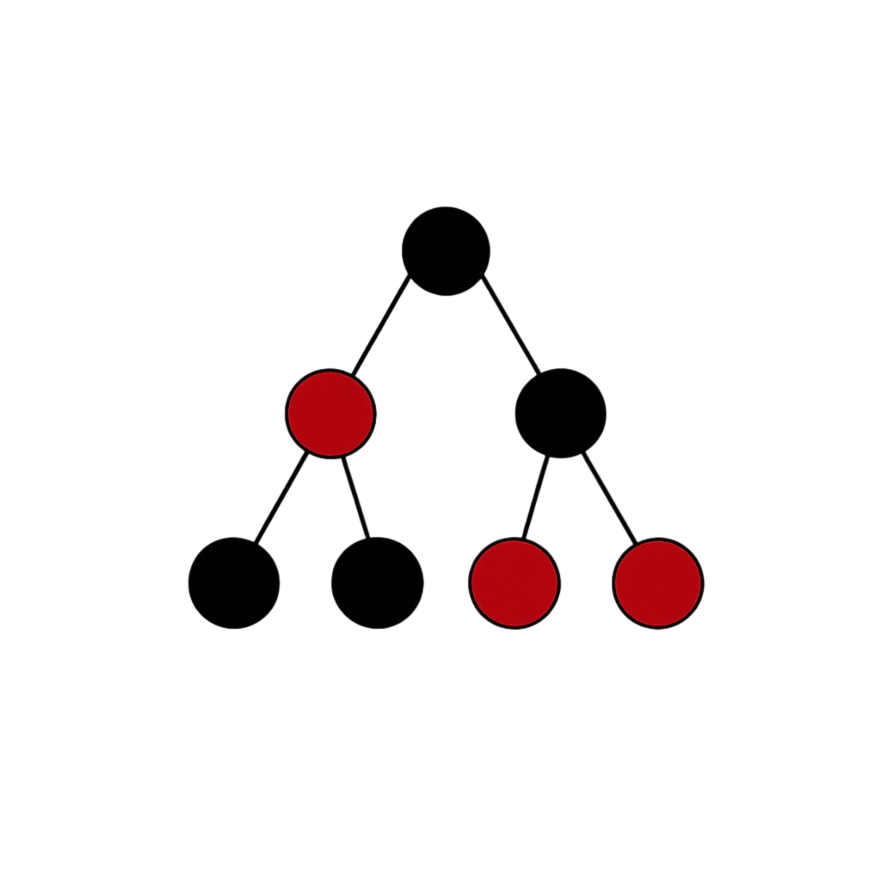
\includegraphics[width=0.38\paperwidth]{kcpc-logo.png}};
    \end{tikzpicture}%
}

\titleformat{\section}{\large\bfseries\color{kcpc-red}}{\thesection}{1em}{}

\setlist[itemize]{noitemsep, topsep=4pt}
\setlist[enumerate]{topsep=4pt}

\title{KCPC Week 1 Problems\\Reasoning Foundations}
\author{}
\date{}

\begin{document}
\maketitle
\thispagestyle{fancy}

\section*{How To Use This Sheet}
Each section has five levels. Start where you are comfortable, but
try at least one problem above your comfort zone. Have a genuine
attempt before looking at the solutions, and use them only when you
are truly stuck. The aim is to learn from the struggle, not merely to
see the answer.

\section{Logic}

\subsection*{Basic -- Same Birthday Month}
There are 13 students in a room. Prove that at least two of them were
born in the same month.

\subsection*{Easy -- Glove Selection}
A drawer contains 5 pairs of black gloves, 3 pairs of brown gloves,
and 2 pairs of grey gloves. You choose gloves in the dark.
\begin{enumerate}[label=(\alph*)]
    \item What is the smallest number needed to guarantee at least one
        matching pair?
    \item What is the smallest number needed to guarantee one matching
        pair of each colour?
\end{enumerate}

\subsection*{Medium -- Three People: Knights, Knaves, and Spies}
Three inhabitants, Alice, Bob, and Carol, each belong to one of
three types: \textbf{Knight} (always tells the truth), \textbf{Knave}
(always lies), or \textbf{Spy} (may tell truth or lie). They make
the following statements:
\begin{enumerate}[label=(\alph*)]
    \item Alice says: ``Bob is a Knave.''
    \item Bob says: ``Carol is a Knight.''
    \item Carol says: ``Alice is a Spy.''
\end{enumerate}
Assuming exactly one is a Knight, one is a Knave, and one is a Spy,
determine who is who.

\subsection*{Hard -- Islander Statements}
Ten islanders each make one statement. Islander $i$ says: ``At least
$i$ of us are liars'', for $i=1,2,\ldots,10$. Every islander is
either a truth-teller or a liar. Which islanders are telling the truth?

\subsection*{Very Hard -- Counterfeit Coin}
You have 12 coins. Exactly one is counterfeit, and it may be heavier
or lighter than the others. Using a balance scale exactly three
times, describe a strategy that always identifies the counterfeit
coin and whether it is heavy or light.

\section{Invariants}

\subsection*{Basic -- Jigsaw Assembly}
A jigsaw puzzle has 500 pieces. A move joins two existing sections
into one larger section. What is the minimum number of moves needed
to assemble the puzzle?

\subsection*{Easy -- Odd Handshakes}
At a party, some pairs of people shake hands. Prove that the number
of people who shook hands an odd number of times is even.

\subsection*{Medium -- Chameleons}
An island has 10 brown, 14 grey, and 15 black chameleons. When two
chameleons of different colours meet, both change to the third
colour. Can all chameleons eventually have the same colour?

\subsection*{Hard -- The MU Puzzle}
Start with the string \texttt{MI}. You may repeatedly apply these rules:
\begin{itemize}
    \item append \texttt{U} to any string ending in \texttt{I};
    \item replace \texttt{Mx} by \texttt{Mxx};
    \item replace \texttt{III} by \texttt{U};
    \item delete \texttt{UU}.
\end{itemize}
Can you obtain \texttt{MU}?

\subsection*{Very Hard -- The Fifteen Puzzle}
The 15-puzzle has tiles numbered $1$ to $15$ in a $4\times4$ frame
with one empty square. The target order has 14 and 15 in the final
two positions. Is it possible to solve the same board if only tiles
14 and 15 are swapped?

\section{Colouring Arguments}

\subsection*{Basic -- One Missing Corner}
Can an $8\times8$ chessboard with one corner square removed be tiled
by dominoes?

\subsection*{Easy -- Corner-To-Corner Knight Journey}
Can a knight start in the lower-left corner of a standard chessboard,
visit every square exactly once, and end in the upper-right corner?

\subsection*{Medium -- Board Walks}
For each board shape below, either find a path that visits every
square exactly once using horizontal/vertical moves, or prove none exists.
\begin{enumerate}[label=(\alph*)]
    \item A cross made from a $3\times9$ rectangle and a $9\times3$
        rectangle sharing their central $3\times3$ square.
    \item The same cross with four squares removed: indexing rows and
        columns from 0 to 8 starting at the top-left corner of its
        $9\times9$ bounding box, remove $(0,3)$, $(3,0)$, $(3,8)$,
        and $(8,3)$.
\end{enumerate}

\subsection*{Hard -- Jumping To The Other Side}
On a $5\times6$ board, a diagonal from the bottom-left to the
top-right corner divides the cells into two sets of 15, marked
\texttt{A} and \texttt{B} below. Initially each \texttt{A} cell has
one counter and each \texttt{B} cell is empty.
\begin{center}
\begin{verbatim}
AAAAAB
AAAABB
AAABBB
AABBBB
ABBBBB
\end{verbatim}
\end{center}
A counter may jump over an adjacent counter to the empty cell
immediately beyond it, horizontally, vertically, or diagonally;
the jumped counter stays in place. Can all counters be moved onto
\texttt{B} cells?

\subsection*{Very Hard -- Domino Tiling Revisited}
For which $n$ can an $n\times n$ chessboard with two missing squares
of opposite colours always be tiled by dominoes?

\section{Induction And Monovariants}

\subsection*{Basic -- Polygon Triangulation}
A convex $n$-gon is divided into triangles by drawing non-intersecting
diagonals. Prove by induction that the number of triangles is always
$n-2$, regardless of the triangulation.

\subsection*{Easy -- Induction Inequality}
Prove that $n!>2^n$ for every integer $n>3$.

\subsection*{Medium -- Infected Chessboard}
A virus spreads on an $n\times n$ board. A square becomes infected if
at least two of its horizontal/vertical neighbours are infected. If
you may choose the initially infected squares, what is the smallest
number with which the whole board can eventually become infected?

\subsection*{Hard -- Parliament Pacification}
In a parliament, each member has at most three enemies. Prove that
the members can be split into two chambers so that no member has more
than one enemy in their own chamber.

\subsection*{Very Hard -- Pebble Spreading}
A pebble starts at $(0,0)$ in the non-negative quadrant of an infinite
grid. A move replaces one pebble by two pebbles in the cells
immediately above and immediately to the right, if both are empty.
Can you clear all
pebbles from the first $n$ diagonals $i+j=0,1,\ldots,n-1$?
Determine all possible positive integers $n$.

\end{document}
